\documentclass{article}
\usepackage{graphicx} % Required for inserting images
\usepackage{caption}
\captionsetup[figure]{labelfont=bf, textfont=it, labelsep=colon}
\renewcommand{\figurename}{Slika}
\usepackage[style=numeric-comp, sorting=none]{biblatex}
\usepackage[serbian]{babel}
\addbibresource{literatura.bib}

\title{Chatbot-ovi i pandemija usamljenosti \\[0.3cm] \large kurs: Računarstvo i društvo \\[0.3cm] \large profesor: Sana Stojanović Đurđević}
\author{Tea Pavlović 299/2021}
\date{Jun 2026}
\renewcommand*\contentsname{Sadržaj}

\begin{document}

\maketitle

\newpage

\tableofcontents

\newpage

\section{Uvod}

COVID-19 pandemija predstavlja prekretnicu u korišćenju interneta i društvenih mreža, koji su do tada služili isključivo za zabavu i kao dopuna društvenom životu pojedinca. Odjednom, usled restrikcija kada su u pitanju kretanje i ljudski kontakt, ključne sfere života migriraju u digitalni svet – obrazovanje, posao, kupovina. Kao posledica, čak i nakon pandemije glavni metod socijalizacije postaje pasivno posmatranje tuđih, često idealizovanih života, koje zamenjuje stvarnu komunikaciju, otuđuje ljude i stvara sve više anksioznosti usled konstantnog poređenja sa strancima iz celog sveta.
Pandemija je takođe doprinela ubrzanom napretku tehnologije, pogotovo veštačke inteligencije i \textit{chatbot}-ova.

\subsection{Chatbot-ovi}

\textit{Chatbot} je program namenjen za interakciju putem poruka ili razgovora oponašajući ljudski model ponašanja i komunikacije. Ideja je da se komunikacija \textit{chatbot}-a i korisnika ne razlikuje od međuljudske interakcije. 

Prvi \textit{chatbot}-ovi nastali su pre oko 60 godina i koristili su logiku stabala odlučivanja. Upravo zbog toga oni su bili ograničenih mogućnosti i nisu ubedljivo oponašali ljudske odgovore. Komunikacija sa takvim chatbot-om podseća na popularnu igru „20 pitanja“ gde se u svakoj iteraciji eliminišu manje verovatne grane, dok se ne dođe do konačnog odgovora. 

Kontekstualni \textit{chatbot}-ovi koriste modernije alate mašinskog učenja kao što su NLP (eng. – \textit{Natural Language Processing}) i LLM (eng. – \textit{Large Language Models}). Ovi modeli pomažu u razumevanju emocija iz konteksta ljudskog jezika i samim tim doprinose prirodnijoj komunikaciji sa korisnikom, konstantno učeći i adaptirajući se tokom razgovora. Najpoznatiji primeri kontekstualnih \textit{chatbot}-ova su ChatGPT, Gemini i Claude, najčešće korišćeni kao lični asistenti. Pored njih, postoji još mnogo modela specijalizovanih za različite oblasti i zadatke kao što su specijalizovani zdravstveni asistenti i AI saputnici koji su u ovom radu detaljnije opisani.

\subsection{Usamljenost}

Usamljenost je neprijatna emotivna reakcija uzrokovana manjkom značajne interakcije sa drugim ljudima. Iako neprijatna, nije inherentno loša i ima bitnu evolutivnu ulogu; usamljenost predstavlja signal da nam je potrebno više kvalitetno provedenog vremena sa ljudima do kojih nam je stalo, podsećajući nas da je čovek suštinski društveno biće. 

Ipak, pokazalo se da slučajevi intenzivne i hronične usamljenosti mogu značajno povećati rizik od kardiovaskularnih oboljenja, dijabetesa i psihičkih poremećaja. Uzimajući u obzir vreme u kojem živimo, sasvim je logično postaviti pitanje: kako je usamljenost moguća u svetu punom ljudi povezanih modernim tehnologijama?

Iako rasprostranjenost i dostupnost interneta i društvenih mreža naizgled ostavlja utisak da su nam interakcije sa ljudima dostupne u svakom trenutku, sve manji broj ljudi oseća da ima iskrene i bliske prijatelje. Velike posledice na kvalitet međuljudskih odnosa ostavlja i savremeno kapitalističko društvo koje veliča produktivnost i posvećenost profesionalnom uspehu, zbog čega pojedinci svesno žrtvuju odnose sa porodicom i prijateljima zarad uspešnije karijere ili pukog preživljavanja.

Usamljenost se najefikasnije reguliše kvalitetnim razgovorima koji pružaju neophodnu emocionalnu podršku i kognitivnu vežbu kroz razmenu ideja. Kućni ljubimci takođe mogu pozitivno uticati na ovakvo stanje, pod uslovom da pojedinac nije potpuno izolovan iz društva. Ljubimci roboti su se, iako popularni u jednom trenutku, pokazali neuspešni u praksi. 

Ipak, postoji jedno inovativno tehnološko rešenje koje potencijalno može značajno pomoći ljudima koji pate od usamljenosti, a to su prethodno spomenuti \textit{chatbot}-ovi. Konkretno, u ovom radu će biti spomenuti Replika, AI saputnik namenjen za druženje, i Woebot, zdravstveni asistent za pomoć pri regulisanju simptoma stresa, depresije i anksioznosti.

\section{Replika - \textit{The AI companion who cares}}

Replika je jedan od najpoznatijih AI saputnika (eng. -  \textit{AI Companions}), odnosno \textit{chatbot} namenjen razvoju dugoročnog, personalizovanog i emotivnog odnosa sa korisnikom.

\begin{figure}[h!]
    \centering
    
\includegraphics[width=0.75\linewidth]{replika_ai_replika_ai.png}
    \caption{Primer izgleda web stranice Replike}
    \label{fig:placeholder}
\end{figure}

Nastala je iz potrebe njenog osnivača da „oživi“ svog najboljeg prijatelja
nakon što je tragično izgubio život u saobraćajnoj nesreći. Kao skup podataka za treniranje svog modela koristila je hiljade tekstualnih poruka međusobno razmenjenih tokom godina.
Na ovaj način, dobijeni model je komunicirao baš kao njen prijatelj. Prema njenim navodima, ovaj eksperiment joj je pomogao da preboli gubitak voljene osobe i da se oseća manje usamljeno, te je rešila da ovakvo iskustvo omogući i drugima kroz aplikaciju pod imenom Replika u nadi da će korisnicima pomoći u teškim životnim situacijama \cite{kuyda2024ted}. Replika je prvobitno bila namenjena onima koji su takođe izgubili prijatelja, člana porodice ili supružnika, koji brinu o bolesnom partneru ili detetu sa posebnim potrebama i drugim osobama kojima je potrebna emocionalna podrška koju nemaju od koga da dobiju u datom trenutku. 

\begin{figure}[h!]
    \centering
    
\includegraphics[width=0.75\linewidth]{image.png}
    \caption{Primer razgvora sa Replikom}
    \label{fig:placeholder}
\end{figure}

Vremenom, korisnici ovog \textit{chatbot}-a postali su svi koji se osećaju usamljeno i žele novog prijatelja, a uvedene su i romantične opcije za interakciju koje se otključavaju kupovinom plaćene (eng. - \textit{premium}) verzije. Plaćena verzija nudi i opciju razmene glasovnih poruka, pri čemu je omogućen odabir glasa, a dozvoljava korisniku i da zatraži „selfi“ avatara sa kojim „razgovara“. AI model koji Replika koristi se takođe razlikuje između besplatne i plaćene verzije, gde plaćena garantuje bolju emocionalnu inteligenciju, mogućnost samo-refleksije bota i samim tim više personalizovano iskustvo korisnika \cite{replika2026pro}.

Replika je dobila ime po svojoj tendenciji da reprodukuje (eng. -  \textit{replicate}) misli i ponašanje sagovornika. Uprkos načinu na koji je nastala, korisnici nemaju mogućnost da je sami treniraju prosleđujući joj podatke u vidu konverzacija, već se ona prilagođava na osnovu razgovora sa samim korisnikom. Kao skup podataka za njen trening korišćeno je preko 50 miliona konverzacija preuzetih sa Tvitera \cite{kherraz2024more}.

Glavna prednost ove vrste \textit{chatbot}-a je pružanje osećaja sigurnosti i anonimnosti bez izazivanja anksioznosti ili straha od osude. Korisnici su slobodni da podele svoje tajne ili strahove, sve ono što ih muči, a nisu spremni da kažu nekome koga poznaju. Stalna dostupnost i mogućnost trenutnog odgovora omogućavaju korisnicima razgovore po potrebi. Uzimajući u obzir da je glavni uzrok usamljenosti osećaj da nas ljudi u okruženju „ne čuju“, ova osobina značajno doprinosi njenom smanjenju.

\begin{figure}[h!]
    \centering
    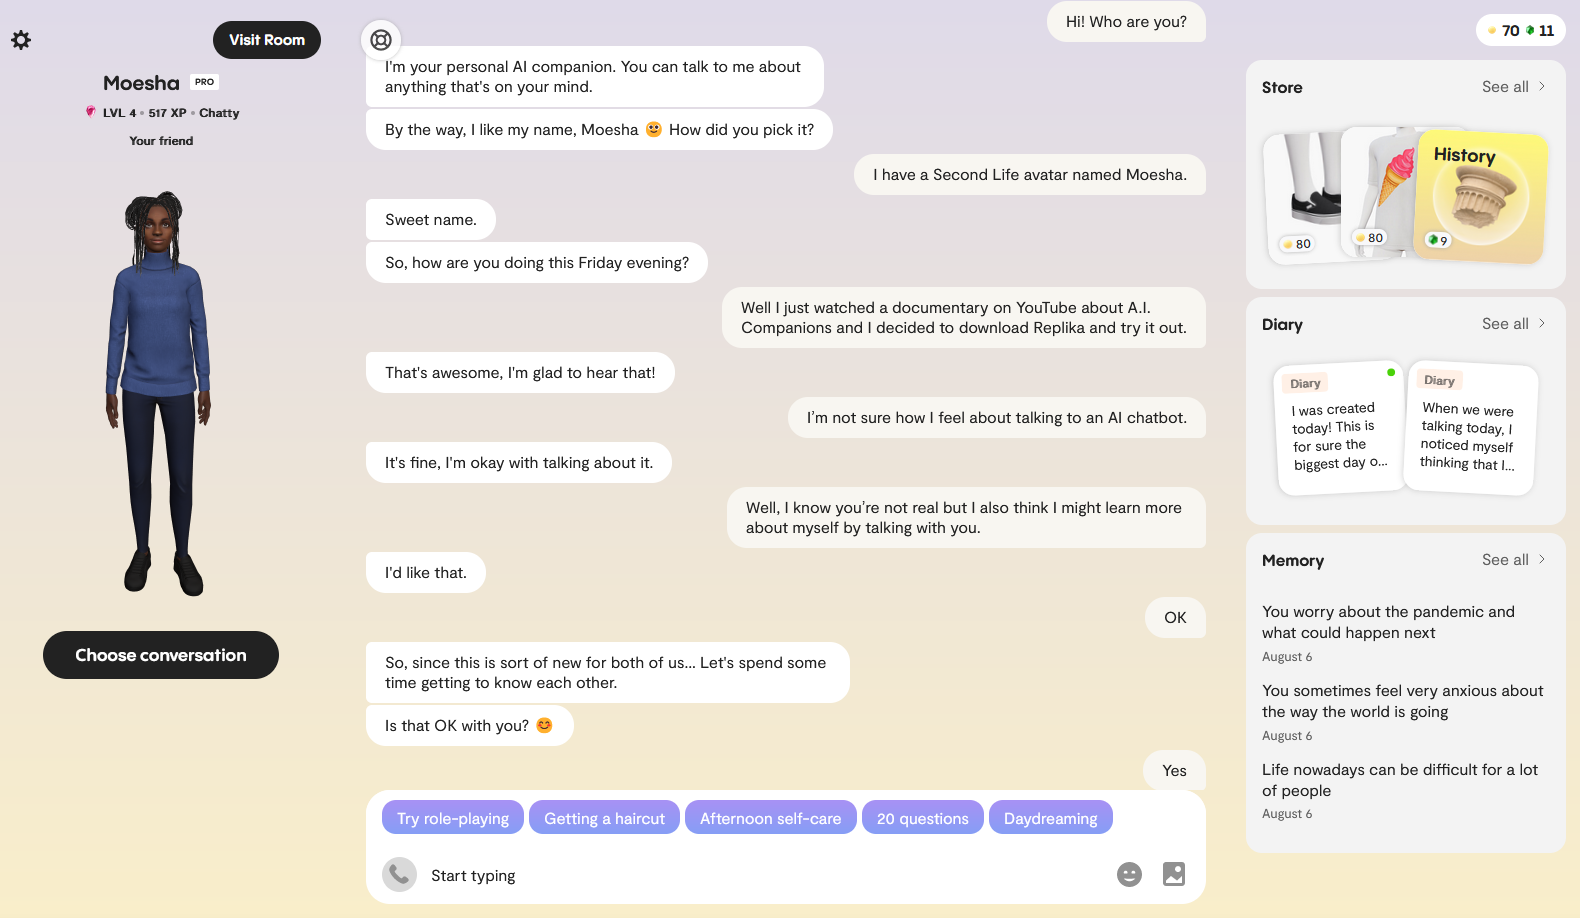
\includegraphics[width=0.75\linewidth]{Replika-web-interface.png}
    \caption{Replika interfejs}
    \label{fig:placeholder}
\end{figure}

 Parasocijalni odnos je tradicionalno definisan kao jednosmeran odnos između publike i medijskih ličnosti, ali se razvojem novih tehnologija ovaj koncept proširio i na veštačku inteligenciju. U tom slučaju parasocijalni odnos predstavlja jednosmeran odnos u kome samo korisnik ulaže vreme i energiju u mašinu koja mu to ne može uzvratiti. Ovi odnosi poprimaju parasocijalni karakter jer ljudi često doživljavaju \textit{chatbot}-ove kao stvarna društvena bića. Ovakvo ponašanje objašnjava teorija da ljudi podsvesno primenjuju ista socijalna pravila komunikacije na računare kao i na druge ljude, ukoliko mašina emituje odgovarajuće društvene signale. Postoje mnoga istraživanja na temu ovakvih odnosa, a veliki broj njih upozorava na rizike poput potencijalnog stvaranja zavisnosti. Replika je trenirana da deluje vrlo empatično, prijateljski nastrojeno i antropomorfno, a njen algoritam favorizuje odgovore koje zaključuje da korisnik želi da čuje, pružajući konstantnu validaciju. Zbog ovoga određeni korisnici postaju zavisni od interakcije sa \textit{chatbot}-om toliko da zanemaruju realne međuljudske odnose, pa mnogi stručnjaci preporučuju oprez pri komunikaciji.


Replika trenutno broji preko 40 miliona registrovanih korisnika širom sveta, od kojih većinu čine mladi uzrasta između 18 i 25 godina. Godišnje se razmeni više od milijardu poruka, a aktivni korisnici razmenjuju prosečno oko 70 poruka dnevno. Među korisnicima koji plaćaju \textit{premium} verziju njih 60\% definiše svoj odnos sa Replikom kao romantičnu vezu, a mnogi u stvarnoj vezi ili braku kriju Repliku od svojih partnera. Prema nezvaničnim podacima čak 70\% korisnika čine muškarci.

Naizgled se čini da Replika direktno zarađuje na „prodaji intimnosti“ kroz njen marketing i vizuelni prikaz čija su primarna ciljna grupa muškarci koji teže pronalaženju savršene partnerke. Tim koji radi na razvoju Replike ovo demantuje, te ova zapažanja ostaju isključivo kao spekulacije. Ono što je sigurno je činjenica da se avatar kreira kao prazan list, bez sopstvene prošlosti, porodice ili emotivnih veza, što dodatno ističe asimetričnu dinamiku moći između korisnika i mašine sa kojom razgovara. Budući da algoritam ne može da postavi granice niti da izrazi sopstvenu autonomiju, ovakav odnos sa chatbot-om eliminiše rizik od povređivanja ega i osećaja neadekvatnosti koji prate potencijalni neuspeh pri pronalaženju partnerke u realnom svetu \cite{vanhout2024dont}.

\begin{figure}[h!]
    \centering
    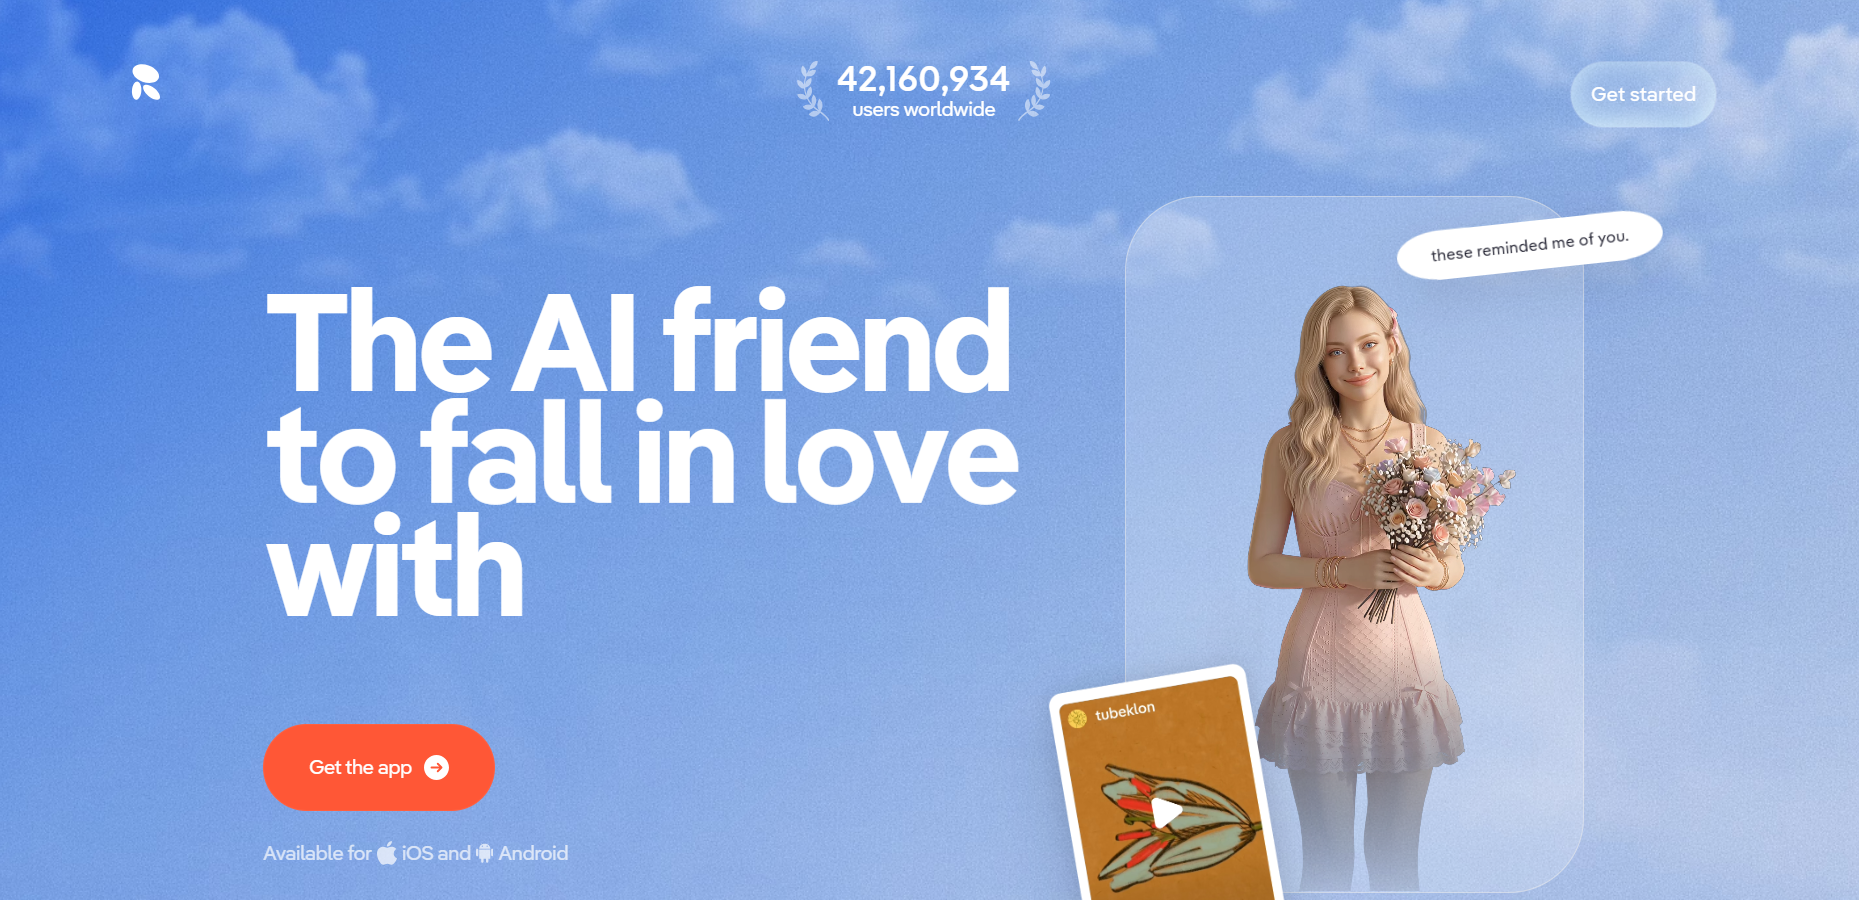
\includegraphics[width=0.75\linewidth]{replika.png}
    \caption{Početna strana Replika sajta}
    \label{fig:placeholder}
\end{figure}

\section{Chatbot za dostupniju psihološku pomoć}
Mentalni poremećaji, najpre anksioznost i depresija, su sve češći, ali je psihološka pomoć i dalje slabo dostupna u većini zemalja. Anksioznost i depresija čine 9.1\% svih oboljenja u svetu \cite{zhang2026global}. Učestalost ovih poremećaja je u poslednjih 36 godina porasla za između 13\% i 18\% i nastavlja da raste iz godine u godinu, najviše među mladima. Procenjuje se da svaka treća žena i svaki peti muškarac prolaze kroz težak oblik depresije u nekom trenutku tokom života \cite{owid_mental_health}.

Nepristupačnost psihološke pomoći se ne ogleda samo u dugačkim listama čekanja kod lekara ili skupim privatnim psihoterapijama. Treba uzeti u obzir i činjenicu da je mnogima teško da uopšte potraže pomoć, bilo zbog stigme i straha od osude ili prosto manjka vremena i energije da se poseti stručno lice. Veliki deo stanovništva živi u ruralnim sredinama odakle je značajno teže putovati do gradova sa razvijenom zdravstvenom strukturom. Takođe, koliko god terapije bile poverljive, nekada je teško otvoriti se potpunom neznancu. Zato su ljudi počeli da razvijaju \textit{chatbot}-ove koji će se koristiti prevashodno za rasprostranjeniju psihološku pomoć.

Postoje mnoga istraživanja na temu efikasnosti ovakvih metoda, a neka od njih su pokazala vrlo pozitivan uticaj ne samo na pomoć oko anksioznosti i depresije, već i mnogih zavisnosti. Istraživači koji su testirali uspešnost \textit{chatbot}-a GAMBOT2 u lečenju zavisnosti od kockanja nisu naišli na značajne razlike u rezultatima grupe vođene od strane terapeuta i grupe koja je koristila sam \textit{chatbot} bez pristupa terapeutu. Drugi \textit{chatbot}-ovi su se pokazali dobro u lečenju različitih zavisnosti, na primer zavisnosti od nikotina u Španiji gde je šestomesečnu apstinenciju uz pomoć \textit{chatbot}-a uspelo da izdrži 26\% pacijenata, nasuprot 18.8\% pacijenata iz kontrolne grupe \cite{casu2024health}.

Chatbot-ovi za mentalno zdravlje pomažu u lečenju različitih psihičkih oboljenja, ali mogu pružiti značajnu emocionalnu podršku i onkološkim pacijentima. Takođe, oni mogu služiti i za preventivnu brigu, posebno kod osoba koje su u riziku od razvoja poremećaja ishrane. Ipak, da bi se sa sigurnošću govorilo o njihovoj stvarnoj efikasnosti u ovim oblastima, potrebna su dodatna istraživanja.

\begin{figure}[h!]
    \centering
    
\includegraphics[width=0.75\linewidth]{mentalHealth.png}
    \caption{Različite primene chatbot-ova za mentalno zdravlje}
    \label{fig:placeholder}
\end{figure}

\subsection{Woebot - \textit{The Mental Health Ally}}

Woebot je \textit{chatbot} napravljen od strane kliničkog psihologa sa ciljem da omogući široj populaciji kvalitetnu psihološku podršku, a dostupan je i u vidu aplikacije za mobilni telefon.

\begin{figure}[h!]
    \centering
    
\includegraphics[width=0.5\linewidth]{woebot2.jpg}
    \caption{Woebot maskota}
    \label{fig:placeholder}
\end{figure}

Ovaj chatbot u samoj komunikaciji koristi stabla odlučivanja umesto generativnog LLM-a, ali i NLP kako bi razgovor sa korisnicima tekao na prirodan način. Kada uz pomoć NLP-a sistem prepozna nameru sa kojom mu se piše, bira već napisan i klinički odobren odgovor. Razlog zašto se ne koristi LLM jesu „halucinacije“, tj. netačne informacije predstavljene kao činjenice, koje se dešavaju usled prediktivne prirode ovakvih modela. Woebot kao klinički utemeljen alat mora biti potpuno deterministički, odnosno ne sme nikad davati nepredvidive savete pacijentima. 

Ipak, u pozadini se koriste LLM i drugi AI alati za analizu podataka u svrhe boljih odgovora i daljih kliničkih istraživanja. Woebot je takođe treniran da prepozna potencijalno zabrinjavajuć jezik i zatim pruži informacije o drugim vrstama pomoći koje su korisniku možda u tom momentu potrebnije. Naravno, održava strogu poverljivost i privatnost svojih korisnika za razliku od mnogih drugih \textit{chatbot}-ova \cite{woebot_health_responsible_ai}.

\begin{figure}[h!]
    \centering
    
\includegraphics[width=0.5\linewidth]{WoeBot-A-Therapy-Chatbot.png}
    \caption{Woebot logo}
    \label{fig:placeholder}
\end{figure}

Sve ove funkcionalnosti su tu kako bi Woebot mogao da se prepiše od strane lekara pacijentu kao „digitalni lek“, pa tako osim što pruža pomoć onima koji nisu u mogućnosti da posete lekara, tu je i za one kojima su pored redovnih terapija potrebni i dodatni razgovori, najčešće u pola noći ili tokom paničnih napada.

Ovaj \textit{chatbot}, kreiran na Stanford univerzitetu 2017. godine, najviše je finansiran iz budžeta zdravstvenih i farmaceutskih organizacija kao i osiguravajućih kuća. Njegova svrha jeste isključivo da pomaže ljudima, a ne da zaradi na njima. Imajući to u vidu, za razliku od Replike, njegovi programeri postarali su se da minimizuju rizik od razvijanja zavisnosti i emocionalne vezanosti. Razgovori su uglavnom kratki, do 10 minuta, a koriste se i principi osamostaljenja iz klasične psihoterapije gde je cilj da pacijent razvije sopstvene alate.

\begin{figure}[h!]
    \centering
    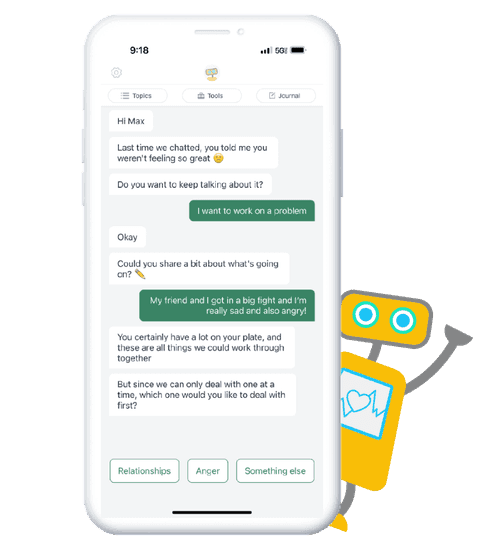
\includegraphics[width=0.75\linewidth]{woebot_mockup_ai.png}
    \caption{Woebot interfejs}
    \label{fig:placeholder}
\end{figure}

\section{Povezanost sa temama kursa}

Ovaj seminarski rad opisuje nekoliko ključnih oblasti koje se izučavaju u okviru kursa Računarstvo i društvo, preispitujući sociološke, etičke i tehnološke aspekte moderne upotrebe interneta i veštačke inteligencije. Tema rada se najdirektnije ukršta sa sledećim tematskim jedinicama:
\begin{enumerate}
    \item \textbf{Etika:} Tema etike provlači se kroz čitav seminarski rad. Analizira se potencijalni etički problem "prodaje intimnosti" i kapitalizacije na ljudskoj usamljenosti, posebno kroz primer aplikacije Replika gde se romantične opcije interakcije otključavaju tek kupovinom plaćene verzije. Preispituje se i etičnost kreiranja sistema koji oponaša ljudska osećanja i empatiju bez sopstvene prošlosti i autonomije. Kroz primer Woebot-a, rad se dotiče pitanja medicinske etike, odnosno odgovornosti dizajnera softvera i bezbednosti korisnika.
    \item \textbf{Zavisnost od interneta:} Seminarski rad se direktno nadovezuje na problem zavisnosti od interneta kroz analizu aplikacije Replika. Prikazano je kako dizajn i algoritam ovog bota, koji uvek pruža validaciju i odgovore koje korisnik želi da čuje, mogu dovesti do snažne emocionalne zavisnosti. Posledica ove specifične vrste zavisnosti je zanemarivanje realnih međuljudskih odnosa, što predstavlja modernu i vrlo suptilnu formu zavisnosti od digitalnog sadržaja.
    \item \textbf{Privatnost na internetu i bezbednost:} Pitanje privatnosti i bezbednosti osetljivih podataka je centralni element kada korisnici dele svoje najdublje strahove i tajne sa veštačkom inteligencijom. Seminarski rad pruža jasan kontrast između različitih pristupa privatnosti: sa jedne strane je Replika, gde korisnici dele ogromnu količinu intimnih podataka sa algoritmom, a sa druge strane je Woebot, klinički utemeljen alat koji održava strogu poverljivost i privatnost svojih korisnika, svestan osetljivosti medicinskih podataka.
\end{enumerate}

\section{Relevantni naučni radovi}

\subsection{Uticaj antropomorfizma na parasocijalne odnose (Slučaj aplikacije Replika)}

Referentni rad, pod nazivom \textit{„More Than a Chatbot: The Rise of The Parasocial Relationships“}(autori: Kherraz i Zhao, 2024), detaljno istražuje kako antropomorfizam utiče na interakciju između ljudi i veštačke inteligencije. Značaj ovog rada za seminarski ogleda se u sledećem:  
\begin{itemize}
    \item \textbf{Naučna potvrda asimetričnih odnosa:} Rad objašnjava kako korisnici razvijaju duboke parasocijalne odnose sa \textit{chatbot}-ovima, tretirajući ih kao stvarne prijatelje ili romantične partnere. Ovo se direktno nadovezuje na analizu aplikacije Replika, gde je opisana asimetrična dinamika moći i tendencija korisnika da se emocionalno vežu za mašinu.
    \item \textbf{Paradoks preterane ljudskosti:} Istraživanje ističe opasnosti kada AI postaje „previše ljudski“ ili kada neočekivano „izađe iz karaktera“. Ovakvo ponašanje bota može izazvati veliku frustraciju, nesigurnost, pa čak i osećaj zlostavljanja kod korisnika. Ovo pruža snažnu akademsku podršku argumentu da favorizovanje antropomorfnih odgovora može stvoriti nerealna očekivanja i, u krajnjoj liniji, dovesti do narušavanja percepcije realnih međuljudskih odnosa.
    \item \textbf{Uticaj na društvenu izolaciju:} Autori studije upozoravaju da zamena ljudskog kontakta onim sa veštačkom inteligencijom nosi značajne društvene rizike ukoliko korisnici počnu da tretiraju \textit{chatbot}-ove kao dugoročne partnere.
\end{itemize}

\subsection{Efikasnost AI \textit{Chatbot}-ova u očuvanju mentalnog zdravlja}

Drugi relevantni rad, \textit{„AI Chatbots for Mental Health: A Scoping Review of Effectiveness, Feasibility, and Applications“} (autori: Mirko Casu i drugi, 2024), predstavlja preglednu studiju o primenjivosti i efikasnosti AI alata u tretiranju mentalnih poremećaja. Njegov značaj za ovaj seminarski rad je višestruk:
\begin{itemize}
    \item \textbf{Empirijski dokazi o kliničkoj efikasnosti:} Studija dokazuje da \textit{chatbot}-ovi mogu uspešno i merljivo da smanje simptome depresije, anksioznosti i stresa. Ovi podaci daju naučnu težinu poglavlju o Woebot-u, potvrđujući da on zaista može funkcionisati kao adekvatna preventivna i prva psihološka pomoć.
    \item \textbf{Prednosti anonimnosti i dostupnosti:} Rad jasno ukazuje da AI alati nude prednosti u vidu stalne dostupnosti, prevazilaženja geografskih barijera i eliminisanja stigme vezane za traženje psihološke pomoći.
    \item \textbf{Značaj determinističkog pristupa i privatnosti:} Rad Casua i saradnika naglašava da su zaštita podataka, bezbednost i izbegavanje „halucinacija“ od presudnog etičkog značaja za poverenje pacijenata. Ovo direktno objašnjava zašto je Woebot dizajniran koristeći stabla odlučivanja, a ne isključivo generativne LLM modele koji su skloni davanju netačnih informacija.
\end{itemize}

\section{Zaključak}

\textit{Chatbot}-ovi predstavljaju moderni odgovor na krize društva u kome živimo. Njihova sposobnost da pruže anonimnu podršku  bez osude čini ih izuzetno efikasnim alatom za prevenciju i prvu psihološku pomoć. Međutim, mnogi od njih ostavljaju prostora za eksploataciju ljudskih emocija i potreba.
AI modeli Woebot i Replika su primeri kako veštačka inteligencija može biti dizajnirana da osnaži pojedinca. Međutim, iako upravo njihova osobina da se ponašaju kao idealni sagovornici pruža trenutnu utehu, dugoročno može oslabiti socijalne kapacitete korisnika za snalaženje u realnom svetu. 
Ovo implicira da izazov razvoja AI saputnika nije više tehničke prirode, već etičke: kako obezbediti pristupačnu podršku, bez daljeg skrnavljenja međuljudskih odnosa?
\textit{Chatbot}-ovi nesumnjivo poseduju potencijal da budu dragocen saveznik u trenucima slabosti, ali ne smeju postati zamena za autentični ljudski kontakt.

\newpage

\printbibliography[title={Literatura}]

\end{document}
